\documentclass[utf8]{../IncArticle}
\graphicspath{{../}}
%\usepackage{color}
%\usepackage{todonotes}
% \usepackage{lmodern}
\usepackage{xcolor}

\colorlet{pcolor}{blue}
\colorlet{fcolor}{red}
\newcommand{\e}[2][fcolor]{\textcolor{pcolor}{[}\textcolor{#1}{#2}\textcolor{pcolor}{]}}
%\def\baselinestretch{2.0}




% *** PDF, URL AND HYPERLINK PACKAGES ***
%
\usepackage{url}

\title{Интерактивная методика извлечения семантической разметки
  текстовых документов, основанная на полисистеме онтологий}

% \AddAuthor{Черкашин}{Е}{вгений}{А}{лександрович}{Институт динамики систем и теории управления СО РАН, Иркутск, ул. Лермонтова 134, 664033}
% \AddAuthor{Черкашин}{А}{лександр}{К}{онстантинович}{Институт географии им. В.Б. Сочавы СО РАН, Иркутск, ул. Улан-Баторская 1, 664033}
% \AddAuthor{Бычков}{И}{горь}{В}{ячеславович}{Институт динамики систем и теории управления СО РАН, Иркутск, ул. Лермонтова 134, 664033}
% \AddAuthor{Паскал}{К}{ристина}{К}{онстантиновна}{Национальный исследовательский Иркутский государственный технический университет, Иркутск, ул. Лермонтова 83, 664074}
% \AddAuthor{Белых}{П}{олина}{В}{асильевна}{Институт динамики систем и теории управления СО РАН, Иркутск, ул. Лермонтова 134, 664033}

\AddAuthor{Черкашин}{Е}{вгений}{А}{лександрович}{}
\AddAuthor{Черкашин}{А}{лександр}{К}{онстантинович}{}
\AddAuthor{Бычков}{И}{горь}{В}{ячеславович}{}
\AddAuthor{Паскал}{К}{ристина}{К}{онстантиновна}{}
\AddAuthor{Белых}{П}{олина}{В}{асильевна}{}

\setcounter{page}{1}
\date{}
\begin{document}

\begin{abstract}
%\boldmath

  Излагается идея подхода к представлению и индукции семантической
  разметки (логического слоя) описания текстового содержимого сайтов,
  юридических документов и т.п.  Этот слой порождается на основе
  анализа вносимых пользователем изменений --- как текстовой
  составляющей, так и его существующей логической структуры.  Варианты
  интерпретации того или иного изменения содержимого (исправление
  ошибки/значения или формирование нового высказывания) уточняются при
  помощи диалога с пользователем.  На принятие решения также влияют
  результаты анализа поведения пользователя, например, выделяются
  повторяющиеся переходы между редактируемыми документами определенных
  классов.  Теоретической основой методики является представление
  предметной области в виде полисистемы онтологий, т.е. расщепленной
  многослойной структуры понятий и отношений, которые отображаются
  между слоями через интерпретацию.

  В качестве тестовой среды для разрабатываемых технологий выбрана
  автоматизация деятельности нотариальной конторы и документооборот
  административных, хозяйственных и научных подразделений бюджетного
  учреждения.  Документы, используемые в этих видах деятельности,
  обладают одним важным свойством --- содержащаяся в них информация
  представляется как в структурируемом, так и в неструктурируемом
  виде.

\end{abstract}

\begin{abstract}[english]\selectlanguage{english}
  A general idea of an approach to representation and induction of a
  semantic markup (logical layer) for description of the text content
  (internet sites, legal documents, and so on) is being described.
  The logical layer is generated on the base of analysis of the
  changes introduced by user.  The changes of the text and the logical
  layer are analyzed.  The variant of the interpretation (e.g., error
  correction of a value or a new statement definition) of the changes
  is determined by means of user interview.  The interpretation also
  depends on the results of analysis of user behavior, e.g., patterns
  of transitions between various kinds of documents.  The theoretical
  basis of the technique is to use of a polysystem representation of
  ontologies for the domain.  The presentation is a hierarchically
  fibered structure of concepts and relations, which are mapped
  between fibers by means of interpretation relations.

  An automation of document preparation activities in a notary office
  and a budgetary institution has been chosen as a testing ground for
  the technologies under development.  The documents that are
  originated and used there have an important common property.  The
  documents contain information which is represented as structural and
  nonstructural data equally likely.

\end{abstract}


\introduction{}

В 2001 году Т.~Бернерс-Ли предложил план развития интернет"=технологий
(семантический веб), который направлен на реализацию сетевых сервисов
со значительным уровнем интеграции логического слоя представляемой
информации.  Информация размечается семантически, а программные
агенты, используя эту информацию, производят ее обработку с целью
решения конкретных практических задач пользователя. Одной из основных
проблем в разработке технологий Семантического Веба (СВ) является тот факт,
что большинство разработчиков интернет-сайтов заинтересованы в решении
своих практических задач, в основном, связанных с представлением
текстовой информации обычному пользователю или другим
интернет-приложениям через подсистемы интеграции данных.
Семантическая интеграция сайтов требует от разработчиков повышения
своей квалификации до уровня, позволяющего использовать эти технологии
в полной мере.  Для того, чтобы ослабить данный фактор необходимо
разрабатывать программные методики семантической разметки содержимого
документов, где сложные технологические аспекты СВ
скрываются от инженера.  Программное обеспечение управления содержимым
сайтов и документооборота должно самостоятельно изымать необходимую
семантическую информацию у пользователя в режиме ``каши из топора''.
Для этого необходимо разработать подсистемы приобретения знаний на
основе диалога с пользователем.

В настоящее время распространены два подхода к семантической разметке
содержимого документа: а) совместное использование формата HTML и RDFa
(Resource Description Framework in Attributes); б) распознавание
интерпретация комбинаций атрибутов HTML некоторым специальным образом
без использования каких-либо расширений HTML.  Первый подход является
результатом планомерного развития технологий СВ.  Сформирован ряд
классов языков представления семантической разметки, различающихся по
выразительности, сложности синтаксиса, сложности алгоритмов обработки,
разрешимости соответствующих им логик описаний (description logics).

Второй подход направлен на создание программной среды обработки
семантических данных, обеспеченных вычислительно несложными
алгоритмами и гарантированной разрешимостью.  Технология микроформатов
\cite{b2:2} --- наиболее известный представитель данного направления.
Микроформатные данные обрабатываются на стороне клиента (в
веб-браузере) при помощи встроенных (plug-in) модулей.  Общими
элементами обоих подходов являются использование HTML в качестве
формата представления текстовой информации, а также использование сетевого
формализма представления знаний для описания логического
слоя и семантической разметки текста.

Общую идею предлагаемого подхода к автоматизации извлечения семантической
разметки удобно излагать на примере юридических документов, которые в
большинстве случаев содержат сведения об отношениях между физическими
и юридическими лицами, а также другими элементами документа.  Эти отношения в
исходной или преобразованной форме используются в других документах.
Поэтому имеет смысл для каждого документа извлекать и хранить
достаточно детально представленное логическое описание таких сведений,
которое преобразуется в текстовый документ при помощи шаблонов.
Вариант преобразования определяется отображаемым документом,
т.е. документ задает контекст представления логического слоя.

К настоящему времени технологии СВ предоставляют формальные механизмы
представления указанных отношений при помощи стандартных форматов и
структур данных, а также несколько механизмов их логической обработки.
Логический слой представления информации в СВ представляет собой граф,
состоящий из концептов (понятий) и отношений между ними.  В частности
в юридическом документе физические и юридические лица находятся с этим
документом в отношении ``часть--целое'', а также в их более точных и
содержательных вариантах.

В настоящее время большинство вариантов использования онтологических
моделей предметных областей в интернет-приложениях сводятся к решению задачи уточнения
диапазона релевантных документов в процессе поиска по ключевым словам
или строке текста.  При этом одной из задач, решаемой в рамках
проблемы является автоматизация извлечения этих моделей из хранимых в сети текстовых
документов.   Для этого производится предварительное сканирование
хранилищ документов и распознавание в тексте метаданных, последовательностей
ключевых слов, построение из этих последовательностей тезаурусов и
т.п., пример --- \cite{irina}.

Наблюдение за поведением пользователей в процессе подготовки различных
документов приводит к заключению, что содержательные части документов,
которые и представляются в логическом слое, как правило, находятся в
тех местах текста, где чаще всего пользователи производят изменения.
Поэтому, информационная система, автоматизирующая такие процессы,
должна отслеживать изменения, вводимые пользователем, во времени и в
пространстве версий.  Версии порождаются копированием документа или
использованием его в качестве шаблона нового документа.  Подвергаться
анализу должна вся совокупность изменений.  Границы изменений
задаются, например, свойствами формата представления текста документа
(гипертекстовой разметкой) или существующей логической структурой
одной из версий документа.
% Предлагаемый подход позволяет сузить объем обрабатываемой информации
% за счет фокусировки алгоритмов анализа данных вблизи изменений.

Элементы логического слоя (концепты, объекты и отношения между ними)
формируются в результате применения алгоритмов анализа данных и
интервьюирования пользователя.  Исходными данными для анализа
выступают следующие структуры\,:
\begin{itemize}
\item полисистема онтологий, совокупно описывающая предметные области,
  имеющие отношение к документу как к структуре данных, так и его
  содержанию;
\item история изменения документа и его логического слоя;
\item список последних изменений в текущей транзакции (новой версии);
\item история действий пользователя в системе в целом\,: пользователь,
  например, выполняет типичный набор действий по подготовке
  стандартного пакета документов;
\item ответы пользователя на утоняющие вопросы системы, цель которых
  --- доопределить точный смысл внесенных изменений.
\end{itemize}

В результате анализа этих данных формируются новый набор троек RDF
вида \texttt{<subject, relation, object>}, представляющих новую
информацию в логическом слое нового документа или его версии.  В общем
случае тройка интерпретируется как отношение (предикат) вида
\texttt{relation(subject,object)}, но, если отношение обладает
функциональными свойствами, то оно может быть проинтерпретировано как
поле некоторого класса \cite{kazakovdiss}, т.е.  \texttt{object =
  subject.relation}.  Логические структуры хранимых в системе
документов необходимо периодически анализировать с целью выявления
отношений, обладающих функциональными свойствами.  Полученные
зависимости представляют собой исходную информацию для принятия
решения об изменении формата представления данных логического слоя.
Например, для набора субъектов одного класса, обладающих одним и тем
же видом функциональных связей, имеет смысл применить реляционные таблицы
в качестве физического хранилища данных, и при этом получить в будущем все
технологические преимущества этого способа хранения данных.  Структура
таблиц проектируется при помощи известного метода функциональных
зависимостей на основе результатов анализа.

Сеть взаимодействующих программных систем, в которых реализованы
перечисленные функции, обладает многими свойствами социальной сети.
Основными видами обработки информации в таких сетях являются ввод,
хранение, фильтрация и передача, т.е. интеграция данных, а не их
агрегация с целью порождения каких-либо комплексных отчетов.  Поэтому
применение специальных методологий проектирования программного
обеспечения при разработке таких систем, например,
объектно"=ориентированных технологий, не является значительным
преимуществом.  Гораздо важнее обеспечить возможность функционирования
программ в доступной недорогой серверной среде (хостинге), а также
необходимо создать стандартные каналы обмена данных с приложениями
других социальных сетей.  Обработку информации агрегированного типа в
социальных сетях выполняют, преимущественно, пользователи и, как
правило, подсознательно.

Интересным свойством такой социальной сети, реализующей, фактически,
распределенный документооборот, является требования к организации
обмена данными между пользователями в процессе подготовки документов
преимущественно в режиме off-line.  Современные информационные
технологии позволяют хранить данные логического слоя в разметке
электронных документов в виде микроформатных данных и RDFa-разметки, а
также в виде QR-кодов, сопровождающих печатные варианты документов.

В качестве платформы для тестирования разрабатываемых технологий
выбрана автоматизация деятельности российского нотариального
офиса.  Операции, выполняемые над документами и шаблонами представимы
как изменения содержания текста документа и его логического
слоя.  Примерами таких операций выступают копирование логического слоя
из одного документа в другой, смена ролей лиц в документа в процессе
его подготовки, накапливание базы данных клиентов и другой справочной
информации, используя упомянутую выше функцию выявления отношений,
обладающих функциональными свойствами.

С целью использования более
простой терминологии в тексте данной работы будем использовать термин
``документ'', обозначая им текстовое содержимое сайтов и документов.

\section{Представление размеченного документа}

Стандартный формат представления знаний RDF описывает информационные
ресурсы при помощи троек вида \texttt{<subject, relation, object>} в
некотором контексте.  Множество всех троек задают некоторый граф
объектов и концептов, а также отношений между ними, формируя
систему знаний предметной области.  Такое описание предметных областей
удобно разбивать на подграфы, организовывать их в иерархические
комплексы \cite{b2:15}, порождая иерархии контекстов.  В общем случае,
контекст влияет на способ или вариант интерпретации троек, например,
отображение фамилии и данных паспорта в разных нотариальных документах
могут значительно отличаться друг от друга.

В предлагаемом подходе \cite{zont2013} шаблоны для отображения
логического слоя документа также хранятся в графе.  При помощи троек
также задаются представления (views) и алгоритмы функциональных
отображений, например, контроллеров (controllers) в рамках шаблона
проектирования MVC (Model View Controller) \cite{b2:5}.  Приведем
пример представления разметки текста (личная информация о человеке) в
формате FOAF (Friend of a Friend), а также часть его шаблонов
представления.

\begingroup%
\tt%
\begin{verbatim}
<rdf:RDF
 xmlns=”http://www.w3.org/1999/xhtml”
 xmlns:rdf="http://www.w3.org/1999/02/22-rdf-syntax-ns#"
 xmlns:foaf="http://xmlns.com/foaf/0.1/"
 xmlns:s="http://www.w3.org/2000/01/rdf-schema#"
 xmlns:view=”http://purl.org/aquarium/engine/MVC”
 xmlns:tal="http://xml.zope.org/namespaces/tal">
  <rdf:Description
     rdf:about="http://www.example.com/People/II/contact#me">
    <rdf:type rdf:resource="http://xmlns.com/foaf/0.1/Person"/>
    <s:seeAlso rdf:resource="http://www.exam..../People/II/contact"/>
    <foaf:homepage rdf:resource="http://www.example.com/People/II"/>
    <foaf:img rdf:resource="http://www.example.com/people/II.png"/>
    <foaf:mbox rdf:resource="mailto:ii@www.example.com"/>
    <foaf:name lang=”en”>Ivan Ivanov</foaf:name>
    <foaf:name lang=”ru”>Иван Иванов</foaf:name>
  </rdf:Description>
  <!— Представление данных физического лица в  HTML+RDFa. -->
  <rdf:Description rdf:about="http://xmlns.com/foaf/0.1/Person">
    <view:pt xml:lang=”ru”>
      <--! Тег view:pt задает формат представления -
           pt (Zope Page Template). -->
      <--! Значение переменной “subj” - это субъект тройки. -->
 <a href=”.” tal:attributes=”href rdf: subj s:seeAlso”
  tal:omit-tag=”not: rdf: subj s:seeAlso”>
       <span tal:replace=”rdf: subj foaf:name”/>
      </a><br/>
 Home page: <a href=”” tal:attributes=”href rdf: subj foaf:homepage”>
  <span tal:replace=”rdf: subj foaf:homepage”/>
      </a><br/>
 E-mail: <a href=”mailto:me@example.com”
           tal:attributes=”href string:mailto:${rdf: subj foaf:mbox}”>
 <span tal:replace=”rdf: subj foaf:mbox”/></a>
    </view:pt>
  </rdf:Description>
</rdf:RDF>
\end{verbatim}%$
\endgroup

В первой части приведенного примера задан экземпляр класса
\texttt{Person} (контактные данные конкретного человека --- Ивана
Иванова) как элемент графа онтологии.  Вторая часть примера ---
описание представления ресурсов класса \texttt{Person}.  В качестве
механизма заполнения текстовых шаблонов данными логического слоя
использована усовершенствованная версия системы Chameleon \cite{q2}.
Механизм интерпретирует результаты выполнения запросов \texttt{rdf:} к
графу как строковые выражения, подставляемые в шаблон HTML, или
заменяющие некоторые исходные конструкции шаблона.  Системе Chameleon передается
набор глобальных переменных, обозначающих отображаемый корневой
субъект (\texttt{subj}), его контекст (\texttt{context}), собственно
сам шаблон (\texttt{template}), а также другие вспомогательные
параметры (\texttt{options}).  В представленном примере \texttt{subj}
указывает на экземпляр класса \texttt{Person}, а \texttt{context}
казывает на документ, в котором упомянут данный экземпляр.  При помощи
переменной \texttt{template} в шаблоне доступны различные константы и
дополнительные данные, которые могут быть использованы в процессе
порождения документа.

Поддержка структур данных троек реализована как расширение синтаксиса
механизма TALES (Template Attribute Language Expression Syntax)
\cite{zopetal}.  Определена новая разновидность выражений
\texttt{rdf:}, общая синтаксическая структура которых соответствует
стандартам RDF (стандартные идентификаторы, пространства имен и т.п.)
и синтаксису языков логик описаний (логические связки, вид выражений).
Библиотека Chameleon также дополнена средствами семантической разметки
порождаемого текста\,: результаты выполнения выражений обрамляются
разметкой данными логического слоя при помощи структур RDFa, что
позволяет, например, передать на сторону клиента информацию о
логическом слое, и использовать ее при формировании пользовательского
интерфейса редактирования документа.

При реализации интерфейса пользователя необходим механизм определения
функциональных отношений алгоритмически.  Для этого в граф вводятся
методы, а также их реализации на разных языках программирования.  В следуем примере при
помощи метода \texttt{nameUpcased} определяется функция представления
имени человека большими буквами.  Для метода заданы две реализации в
языках Python и JavaScript.

\begingroup
\tt
\begin{verbatim}
<rdf:RDF xmlns:html=”http://www.w3.org/1999/xhtml”
  xmlns:rdf=http://www.w3.../22-rdf-syntax-ns#
  xmlns:foaf="http://xmlns.com/foaf/0.1/"
  xmlns:s=http://www.w3..../rdf-schema#
  xmlns:view=”http://purl.org/aquarium/engine/MVC”
  xmlns:tal="http://xml.zope.org/namespaces/tal">
  <rdf:Description rdf:about="http://xmlns.com/foaf/0.1/Person">
    <view:method html:id=”nameUpcased”>
       <html:script type="text/python" xml:lang=”ru”>
  <--! Экземпляр передается в параметр “self” -->
   return self[“foaf:name”][0].upper()
       <html:script>
       <html:script type="text/javascript" xml:lang=”ru”>
  <--! Экземпляр задается переменной “this” -->
   return this.query(“foaf:name”)[0].toUpperCase()
       <html:script>
    </view:method>
  </rdf:Description>
</rdf:RDF>
\end{verbatim}
\endgroup

Ограничение прав доступа также реализуются по аналогии с
представленным в \cite{b2:6,b2:7}, используя данные, представленные
также в виде троек RDF.

Содержимое документа, в общем случае, представляется в виде дерева,
где большинство узлов являются и субъектами и объектами
одновременно. Исключения составляют корневой узел (он является только
субъектом) и листовые узлы (только объекты).  В иерархии документов
корневые узлы документов связаны другими отношениями, например,
организацией документов в тематические иерархии и кластеры.

\section{Извлечение разметки документа} \label{sec:markupproc}

% Одним из основных моментов исследования --- это разработка методики
% адаптации процесса извлечения разметки к процессу редактирования
% документа.
Изменения документа представляются двумя вариантами интерпретации\,:
изменение поля \texttt{object}, что соответствует тривиальному
исправлению ошибки или исправлению текста шаблона; содержательное
изменение, приводящее к формированию нового отношения между каким-либо
субъектом в контексте документа и изменяемым значением (объектом).
Далее будем рассматривать только изменения, которые влияют на
содержательный смысл документа, соответственно изменяя его логический
слой.
% Анализ изменений в тексте документа направлен на формирование новых
% данных и знаний, при этом система играет активную роль, а
% пользователь является источником дополнительной информации.

Обогащение семантической разметки осуществляется в среде, содержащей
логическую структуру исходного документа, которая уже храниться в базе
данных.  И тогда перечень данных, используемых системой для принятия
решения о том, какой вид будет иметь новая тройка, включает следующие
источники информации\,:
\begin{enumerate}
\item онтологическая модель предметной области;
\item исходная версия документа;
\item изменения текста документа, представленные в виде стандартного
  diff-формата \cite{diff};
\item ответы пользователя на вопросы, задаваемые системой; ответы
  уточняют намерения пользователя;
\item перечень действий пользователя, предшествовавших данному
  исправлению документа. \label{em:behav}
\end{enumerate}
Суть п.~\ref{em:behav}, например, проявляется при создании нового
документа из шаблона или его копии, что, вообще говоря, приводит к
необходимости заполнения определенного перечня полей \texttt{object}
уже существующих троек.  Таким набором, например, выступает
стандартный набор полей для идентификации физического лица (ф.и.о.,
данные паспорта, адрес места жительства и т.п.) в нотариальной
доверенности.  Другим примером выступает подготовка целого пакета
документов, в которых используются одни и те же физические и
юридические лица.

Если же документ модифицирован частично, то данное изменение
интерпретируется как уточнение логической структуры документа или
другого субъекта, т.е. как создание нового отношения с некоторым объектом.
Такие изменения приводят к созданию новой тройки, соединяющей
существующий субъект и новым значением-объектом, при этом пользователю
необходимо выбрать \texttt{subject} для этой новой тройки.

Новый субъект должен быть выбран из списка (дерева) всех существующих
в контексте документа субъектов.  Далее для этого субъекта формируется
список выбора отношения, который формируется из всех возможных
отношений для этого субъекта и его класса, включая классы-предки.
Пользователю необходимо выбрать одно отношение для формируемой тройки.
Если в списке не содержится подходящего отношения, то его необходимо
определить.  Новое отношение всегда уточняет какое-либо уже
существующее в списке отношение.  Чтобы контролировать приумножение
сущностей без необходимости, необходимо периодически проводить анализ
существующей иерархии отношений инженерами знаний.  Их задача ---
исключить дублирующие (эквивалентные), противоречивые и семантически
неточные отношения, и производить реорганизацию (refactoring)
онтологической модели.

При удалении объекта какой-либо тройки, вся тройка должна быть также
удалена из логического представления документа.  Процесс удаления
должен контролироваться анализом минимальной структурной полноты и
семантической непротиворечивости субъекта (иерархии субъектов).
Например, при удалении из договора физического лица, должны быть
удалены и его паспортные данные. В результате анализа либо удаление
разрешается, либо запрещается, либо создает цепочку удалений троек,
как в примере с физическим лицом.  Для реализации этой функции каждый
класс субъектов необходимо сопроводить перечнем троек, которые
необходимы для формирования его содержательного базиса.

Добавление целого набора троек (подграфа), например при копировании
части размеченного документа, в общем случае, приводит к
добавлению новых субъектов и отношений в контекст.  Примером такой
ситуации выступает создание трехстороннего договора из двустороннего
добавлением нового физического лица.  При этом также необходимо, в
общем случае, заполнить необходимые поля паспортных данных, а также
установить отношения между контекстом, субъектами документа и новым
физическим лицом.

\section{Теоретическое обобщение процесса извлечения разметки}

Вышеописанный процесс является тривиальным вариантом пошаговой
реализации процедуры полисистемного анализа и синтеза \cite{father}
(ППАС) в приложении к декомпозиции предметной области документа. ППАС
является обобщением процедуры системного анализа предметных областей.
Суть процедуры состоит в том, что предметная область и все ее объекты
и процессы расщепляются по солям и представляются концептами и
отношениями (морфизмами) в многомерном пространстве.  В отличие от
классического системного подхода, где принцип взаимодействия элементов
является фундаментальным, полисистемный анализ предполагает выполнение
гипотезы расслоения, т.е. он предполагает, что
\begin{enumerate}
\item объект исследования представим в виде заимонепересекающихся
  слоев (в частном случае, подмножеств), подобластей. \label{req1}
\item концепты и морфизмы одного слоя должны отождествляться с
  концептами и морфизмами во всех других слоях через явное или неявное
  отношение интерпретации (подстановки). \label{req2}
\end{enumerate}
Таким образом, полисистема является системой сама по себе с более
общей точки зрения, а ППАС --- это новый вид системного анализа.

В общем виде приложение ППАС к задаче автоматизации построения
разметки документов состоит в построении многослойной декомпозиции
предметной области и данных документа. В качестве слоев выступают
различные аспекты представления документа\,: структурная
(мереологическая) организация документа, концептуальное моделирование
предметной области документа, наследование свойств документов,
моделирование отношений между физическими и юридическими лицами,
модели документов в деонтической логике и т.п.  В идеальном случае в
каждом слое в результате выполнения процедуры ППАС должна быть
построена законченная теория, представленная в виде полного набора
концептов и морфизмов.  Требование (\ref{req2}) в вышеупомянутом
списке позволяет организовать процедуру обеспечения полноты
синтезируемого слоя в процессе декомпозиции, проверяя его
тождественность существующим полным слоям.

%Таки для обеспечения необходимой производительности системы
%достаточно проверять тождественность не всем слоям, а только тем,
%которые объявлены как "шаблоны" или "теории".

Благодаря (\ref{req2}) теории каждого слоя являются схожими через
интерпретацию, не смотря на то, что отличаются друг от друга своими
фундаментальными основаниями.  Это позволяет индуцировать (порождать)
новые аксиоматические теории предметных областей по образу и подобию
уже существующих.  Каждый системный уровень (слой) знаний также
многократно и последовательно расслаивается, порождая полисистемное
представление исследуемого объекта.  Таким образом, все системные
теории комбинируются в объединенную модель, описывающую и предметную
область и объект исследования.  Интерпретация данного свойства ППАС в
нашей задаче представляется нам как обобщение процесса декомпозиции
предметной области документооборота и проектирования информационной
системы через расслоения понятий и интерпретацию существующих
алгоритмов, реализующих теорию некоторого слоя, в алгоритмы других
слоев.

В нашем случае ППАС направлена на формирование троек и контекстов
(слоев).  Получаемые классы документов, физических и юридических лиц,
а также других объектов, формируют множество концептов теории
соответствующего слоя.  Выделяя новый класс или отношение между
классами, необходимо установить (алгоритмически, логическим выводом,
выводом по аналогии или анализом ответов пользователя) связь с
концептами и отношениями в других слоях (интерпретацию).  Для удобства
восприятия получаемой логической структуры необходимо также задавать
для получаемых концептов определения на естественном языке,
соответствующее слою.  Требование наследования свойств отношений в
процедуре извлечения разметки (см. раздел \ref{sec:markupproc}),
отнесение некоторого субъекта к классу, построение различных иерархий
классов --- это примеры реализации интерпретаций понятий между слоями.

Таким образом, применение ППАС позволит решать задачи обеспечения
полноты системы объектов, понятий и отношений в документе, верификации
непротиворечивости и, в далекой перспективе, автоматизации порождения
программ, реализующих теории слоев через интерпретацию существующих
алгоритмов, а также позволит реализовать много других сервисных
процедур.

\subsection{Ведение диалога с пользователем}

Рассмотрим пример использования полисистемы онтологий в реализации
диалоговой подсистемы интервьюирования пользователя (ДПИП).

Для реализации ДПИП необходимо, чтобы в системе уже были реализованы
слои представления отношений ``часть-целое'', иерархии классов
сущностей, наследование отношений между классами и объектами, теория
множеств и некоторые предметные слои, например, слой, определяющий,
что мужчины и женщины --- это непересекающиеся множества людей.  Цель
диалога с пользователем --- выделить установить принадлежность нового
объекта некоторому контексту (слою), установить его интерпретацию в
концепты других слоев, а также установить полный набор
непротиворечивых отношений с объектами контекста.  Диалог с
пользователем строится на основе анализа известных свойств и
ограничений над объектом\,: тип данного, местоположение исходного
субъекта в иерархиях контекстов, существующие отношения с другими
объектами и др.

% Свойство отображения концептов между слоями через интерпретацию
% \e{должно быть использовано} в качестве основы реализации диалоговой
% подсистемы взаимодействия с пользователем.  При этом при помощи
% рассуждения по аналогии, представляемое в полисистеме онтологий как
% анализ структуры отношений в слое и движение вдоль отношений и
% интерпретационных отображений (между слоями).  \e[cyan]{Похоже на
% повторение при прямом прочтении текста статьи.}

Рассмотрим простой пример модели семейных отношений, изображенный на
рис.~\ref{OPSA} (на рисунке большинство очевидных отображений
интерпретации не отображены).  Полисистема, изображенная на рисунке,
включает четыре слоя, которые представляют собой различные модели
семьи Боба.  Слой 1 представляет семью как конкретный объект, в этом
слое содержатся только конкретные объекты.  Слой 2 задает основные
роли (отношения) членов семьи. Слой 3 представляет понятие ``пол'' как
две взаимоисключающие противоположности.  Слой 4 отображает
мереологическую концепцию, т.е. суть отношения ``часть--целое''.

Попробуем построить на основе этой полисистемы онтологий список
вопросов, при помощи которых определяется, какую роль в семье Боба
играет Джул.  Предположим, что уже известно, что Джул --- женщина.
Чтобы поместить Джул в слой 1 необходимо задать вопрос пользователю\,:
``Является ли Джул частью семьи Боба?''.  Вопрос порождается в
результате индуктивного вывода о том, что все отношения в семье через
интерпретацию отображаются на отношение ``partOf:'' слоя 4.  Это
заключение моделируется контравариантным функтором из слоя (категории)
2 в слой 4 (показано на рисунке стрелкой от отношения ``бытьОтцом:'' к
``partOf:'', другие аналогичные стрелки не изображены).  Теперь для
того, чтобы подтвердить факт, что Джул --- член семьи Боба достаточно
спросить\,: ``Правда ли, что Джул являетьсяЧастью: Семьи Боба?''.
Обозначение экземпляра ``Семья'' можно сформировать по традиционному
принципу обозначения семьи именем отца семейства (ОС), т.е. именем
``Боб''.  Данный факт обозначен на рисунке стрелкой от Боба в слое 1 к
концепту ``ОС'' слоя 2.

Если пользователь ответил на данный вопрос утвердительно, т.е. Джул
является частью семьи Боба, то нам нужно далее уточнять роль Джул, так
как отношение ``partOf:'' не используется в явном виде в слое 1.  Джул
--- женщина, поэтому не может быть ни отцом не сыном. Если бы это было
так, то она должна быть мужчиной, но мужчина и женщина --- формально
противоположные концепты.  Если для отношения ``бытьМатерью:'' в слое
1 задана кратность, то уже будет известно, что в семье уже есть мать
Алиса.  Поэтому остается один вариант задать вопрос:''Джул [играет
роль] дочери в семье Боба?''.  И теперь, если ответ будет
утвердительный, то создается новая тройка: \texttt{<Bob's-family
  hasDaughter: Jul>}. Если, например, пол Джул неизвестен, то второй
вопрос синтезируется следующим образом: ``Какую роль играет Джул в
семье Боба?''.  В качестве вариантов ответа выдается список из двух
отношений: ``hasDaughter:'' and ``hasSon:''.

На самом деле в первоначальном примере первый вопрос задавать нет
необходимости, т.к. в семье осталась только одна роль для женщины.
Если, например, убрать из слоя Алису, мать, то в этом случае в первом
вопросе появляется смысл.  Вопросы общего характера задаются там, где
необходимо сузить количество альтернатив в ответах в будущем.  Кроме
того, последовательность вопросов можно определять аналогично дереву
решений.

\e{проверить соответствие картинки тексту, принять решение о русском
  или английском названии отношений.}

\begin{figure}
\begin{center}
\sf
\def\svgwidth{0.7\linewidth}
\input{layer.pdf_tex}
\end{center}
\caption{Пример использования полисистемы онтологий \e{проверить
    эргономичность картинки}}
\label{OPSA}
\end{figure}



% (HERE: a generalizing resume paragraph needed.  )

% (About polysystem of ontologies).

% (procedure of fibration)

% (procedure of completeness reconstruction): (About mapping via functors).

% (Induction of notions, suppositions of fibrations).

% (wikipedia and Google search systems).

% (!! Systems of complexes. !!)

\section{Приложение методики в нотариальном офисе}

Приложением методики и разрабатываемых технологий является
автоматизация процесса подготовки нотариальных документов.
Текст документов включает как формализованную, так и неформализованную
информацию в соотношении, удобном для наших исследований.  К
формализованной информации, например, относятся паспортные данные
физического лица, данные регистрации транспортных средств и т.п.
Формализованные части документов активно передаются из документа в
документ, хранятся в базах данных реляционного типа, при этом эта
информация формирует цепочки нотариальных действий в один шаблонный
процесс.  Окончательная структура нотариального документа, в общем случае,
определяется данными формализованной части текста.
Например, формат нотариальной подписи зависит от дееспособности
упомянутых в документе физических лиц.

В настоящее время документы порождаются из шаблонов.  Шаблоны
документов в экспериментальном офисе подготавливаются инженером
совместно с секретарями\,--\,заместителями нотариуса, имеющими
достаточный опыт работы с имеющейся системой.  Шаблон представляет
собой HTML-форму, встроенную в текст документа.  Логическая структура
задается именами полей, а алгоритмы обработки информации не выходят за
рамки стандартных технологий разработки интернет-сайтов.
Результирующий документ порождается при помощи замены полей формы на
введенные значения.  Неформализованная информация в нотариальных
документах представляется в виде абзаца текстов, ссылки на статьи
кодексов, разъясняющий текст и т.п.  Имена полей форм обозначены
идентификатором специальной структуры, позволяющей соотнести наборы
полей в отдельный субъект, который они описывают.  Такая простая
формализация уже позволяет выполнять базовые операции по
преобразованию роли субъекта в документе через переименование частей
идентификаторов, передавать (копировать) данные формы из одного
документа в другой.

Применения разрабатываемого подхода призвано повысить уровень
автоматизации сотрудников нотариальной конторы, в части автоматизации
разработки шаблонов документов. Необходимо вовлечь секретарей,
сотрудников с невысокой инженерной квалификацией, в процессы
формирования базы шаблонов документов и их классификаций, а также
представить основу обмена личными данными физических и юридических лиц
между нотариальными конторами.

% Логический слой нотариальных документов состоит из иерархии субъектов
% \e{как это уже неоднократно было сказано выше}.  Все эти субъекты
% находятся друг с другом в различных отношениях в различных слоях
% \e{и об этом также мы уже неоднократно говорили выше}.  Например, в
% доверенность включает по крайней мере два физических лица\,: одного
% \e{доверенного} и одного \e{доверяющего}.  Для каждого физического
% лица в документе представлены паспортные данные и место проживания.
% Доверенность может содержать также другую личную информацию, например,
% о частично дееспособных детях.

Рассмотрим пример представления логического нотариальной доверенности
в рамках предлагаемых технологий СВ.  Стороны в доверенности
формализуются тройками \texttt{<letatt998 containsPrincipal: indiv78>}
и \texttt{<letatt998 containsProxy: indiv79>}, где \texttt{letatt998},
\texttt{indiv78} и \texttt{indiv79} --- идентификаторы конкретного
документа и конкретных физических лиц.  Оба отношения
\texttt{containsPrincipal:} и \texttt{containsProxy:} являются
специализациями абстрактных отношений \texttt{hasIndividual:} и
\texttt{partOf:}, предназначенных для определения объектов некоторого
класса и структурных элементов документа.  Теперь, используя
неразличимость отношений \texttt{containsPrincipal:} и
\texttt{containsProxy:} в одном из слоев можно в интерфейсе
пользователя установить элемент управления, который в документе меняет
отношения \texttt{containsPrincipal:} на \texttt{containsProxy:} (и
наоборот) в соответствующих тройках.  В общем виде верхний уровень представления
нотариальных документов представлен на рис.~\ref{notaryontology}.
\begin{figure}[!t]
\centering
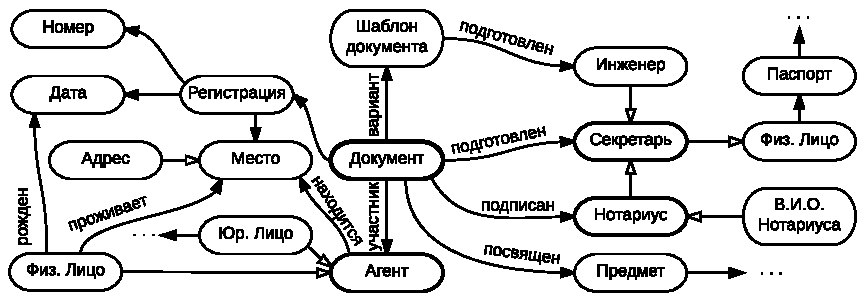
\includegraphics[width=0.8\linewidth]{DocumentOntology-ru.pdf}
% where an .eps filename suffix will be assumed under latex,
% and a .pdf suffix will be assumed for pdflatex; or what has been declared
% via \DeclareGraphicsExtensions.
\caption{Верхний уровень онтологии предметной области представления
  нотариального документа}
\label{notaryontology}
\end{figure}


\section{Архитектура программной системы и средства реализации}

Программная система разрабатывается как интернет-приложение с
возможностью установки локальной версии на персональный компьютер
пользователя.  На рис.~\ref{architecture} представлена общая
архитектура ядра программной системы.  Ядро построено на популярной
клиент-серверной архитектуре.  Клиент с сервера получает результат
применения шаблона Chameleon к некоторому объекту (модуль ``Генератор
вида'').  Для этого необходимо загрузить этот объект, что
обеспечивается модулем ``Загрузчик троек''.  Объект представляется
набором его троек; порождаемый текст включает только те данные,
которые разрешены для просмотра данному пользователю.  Доступ к данным
контролируется в модуле ``Защита данных''.  Отфильтрованные тройки не
отображаются, при этом пользователю выдается соответствующее
информационное сообщение.  Задача модуля ``Диспетчер представления
данных'' предоставлять система сервис хранения троек в различных
форматах представления данных, преобразовывать тройки в эти форматы и
обратно.  Использование нескольких форматов позволяет поддерживать
алгоритмически различные агрегатированные операции над данными.
Например, регистрационные данные транспортных средств удобно хранить в
реляционной базе данных и использовать соответствующие средства для
осуществления быстрого поиска.  Примером хранилища, поддерживающим
различные форматы данных, выступает OpenLink Virtuoso Universal Server
\cite{b2:8} и его свободная версия.

\begin{figure}[!t]
\centering
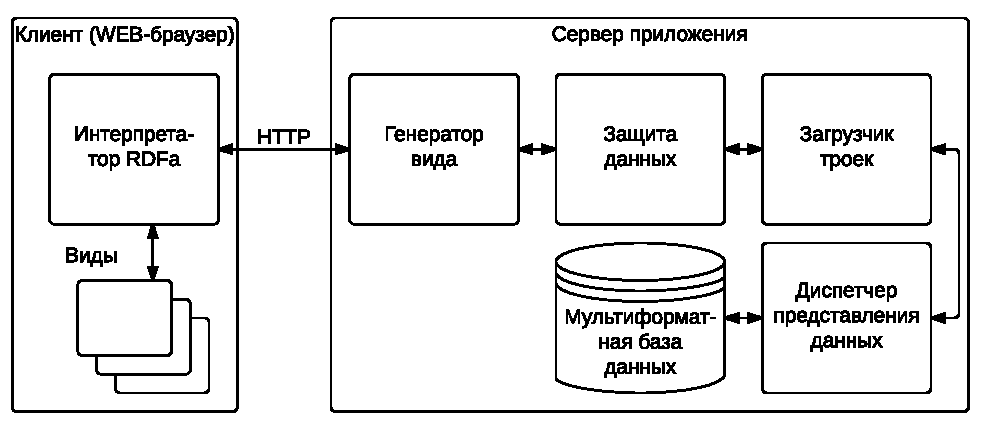
\includegraphics[width=0.8\linewidth]{peixe-architecture-ru-1.pdf}
\caption{Архитектура программной системы}
\label{architecture}
\end{figure}

\subsection{Используемые инструментальные средства}
\label{sec:instr}

Ориентация проекта на решение прикладных задач приводит к следующему
набору требований к целевым свойствам программного продукта.
\begin{enumerate}
\item Программная система должна относится к классу свободного
  (open-source) программного обеспечения. Цель --- привлечь
  общественность к проблеме разработки и (ре)инжениринга
  документооборота как полисистемы онтологий.
\item Программа должна иметь две реализации\,: локальную и в виде
  интернет-приложения. При этом будет обеспечен максимальный охват
  пользователей как открытой части сети, так и закрытой.
\item Северная часть интернет"=приложения должна быть нетребовательна
  к вычислительным ресурсам и функционировать в среде недорогого
  разделенного хостинга (shared hosting).  \label{e12:p2}
\item В следствие п.~\ref{e12:p2} необходимо обеспечивать поддержку
  различных систем хранения данных для хранения троек.
\end{enumerate}
% Современные ресурсы, предоставляемые коммерческими
% интернет"=провайдерами, ранжируются от предоставление ресурсов для
% процесса веб"=сервера до виртуального и облачного хостинга.  Недорогим
% классом является первый вариант, называемый виртуальным хостингом.
В качестве популярной платформы в разделенном хостинге выступает
комбинация языка программирования PHP, сервера баз данных MySQL,
функционирующих под управлением операционной системы Linux.  Кроме
того, современные интернет"=приложения на стороне веб-браузера активно
используют среду программирования JavaScript.

Представление графа семантики в PHP, а также доступ к его компонентам,
обеспечивается библиотекой EasyRdf.  Библиотека позволяет загружать
графы в формате RDF. Библиотека позволяет представлять граф в виде
объектов PHP, к которым обеспечивается доступ в
объектно"=ориентированном стиле, или при помощи стандартного языка
запросов SPARQL.

Хранение RDF"=троек в реляционной базе данных MySQL поддерживается
библиотекой ARC2, которая также реализует язык запросов к
RDF"=графу SPARQL.  ARC2 представляет собой платформу разработчика
приложений с функциями СВ, которая поддерживает расширение базовых
функций встраиваемыми модулями, создание триггерных функций на
обработку результатов запросов SPARQL.

% Также для реализации системы может быть полезна библиотека Redland,
% предоставляющая высокоуровневый интерфейс для работы с RDF. Redland
% позволяет загружать RDF"=граф из XML"=файла, обеспечивает его хранение
% и обработку. Данная библиотека имеет объектно"=ориентированную
% модульную структуру и поставляется с детальной справочной
% документацией и примерами применения. Предоставляются API для языков
% C"=Шарп, C, Perl, Python, Ruby, PHP, Java и Tcl. Redland поддерживает
% различные RDF"=словари, включая FOAF, RSS 1.0, Dublin Core, DOAP и
% OWL. Приемущество данной библиотеки состоит в том, что она поддерживает хранение графов с помощью различных СУБД, таких как Sleepycat/Berkeley DB, MySQL, PostgreSQL и др.  \url{http\,://www.filewatcher.com/d/Debian/sparc/libs/librdf"=storage-postgresql_1.0.10"=3_sparc.deb.38502.html}

Использование технологий ZOPE Page Template (ZPT) в качестве основного
механизма порождения текста из логического слоя позволяет независимо
от платформы реализации системы представлять форму отображения троек,
при этом хранить ее в самом графе.  ZPT --- это система шаблонов,
которая позволяет программистам и дизайнерам создавать динамические
WEB-страницы.  Первоначально ZPT являлся частью системы ZOPE и получил
достаточную популярность вследствие своего декларативного подхода к
описанию трансформации HTML- и XML-документов.  В состав технологии
входят интерпретаторы языков запросов к логическим структурам языка
программирования TALES (Template Attribute Language Expression
Syntax), методы обработки древовидного представления гипертекстовых
документов METAL (Meta TAL), а также средства интернационализации
(I18N).  Разработчики ZPT преследовали целью решить следующие
стандартные для WEB задачи:
\begin{enumerate}
\item Обеспечение разделения пользовательского интерфейса и логики приложения;
\item Создание пользовательского интерфейса при помощи обычных файлов HTML, что позволяет разработчикам использовать специальные программные пакеты для редактирования и разработки Web-сайтов (например, Dreamweaver);
\item Избавление пользователя от реализации циклов для заполнения таблиц и элементов списка;
\item Управление отображением элементов Web-страницы в зависимости от свойств данных.
\end{enumerate}

В настоящее время существует множество реализаций
интерпретаторов TALES и METAL для различных систем программирования, в
том числе для языка программирования PHP существует реализация данной
системы – PHPTAL, поддерживающая пространства имен TALES, METAL и
I18N.  Базовый синтаксис и семантика языка TALES является независимым
от языка реализации библиотеки, что является одним из факторов
переносимости всей технологии.

Для подпрограмм JavaScript, функционирующих на стороне веб-браузера,
функции ZPT реализуются при помощи библиотеки Distal, которая
позволяет подгружать данные в шаблон динамически.  Это позволяет
разработчику интернет-приложения переносить часть функций отображения
документа на сторону клиента, т.е. задействовать вычислительные
ресурсы рабочей станции и разгрузить сервер.

Локальные  пользовательские версии приложения должны быть просты в установке,
настройке и сопровождении, поэтому хранение логического соля в СУБД
коммерческого ровня, таких как DB2, Oracle или Microsoft SQL Server,
не является целесообразным, т.к. требую к себе профессиональное
внимание на этапах установки и сопровождения.  Более удачным вариантом
для хранения данных являются встроенные в основной процесс системы
управления базами данных, не требующие обеспечения специальных форм
межпроцессного взаимодействия.  Как правило такие системы также предельно
просты на этапе установки и конфигурирования.

Одним из интересных примеров такой СУБД является система Kyoto Cabinet
\cite{kyoto}, представляющая собой библиотеку процедур для управления
базой данных в стандарте BerkeleyDB. Библиотека хранит данные в одном
или нескольких файлах в файловой системе, обеспечивает эффективное
отображение уникальных ключей на значения.  И ключ и значение являются
нефиксированными последовательностями байтов.  Отображения
организованы при помощи хэш"=таблиц или B+-деревьев.  Кроме этого,
Kyoto Cabinet реализует различные методы защиты информации от утери
вследствие физических нарушений носителя\,: разреженный формат данных
с дублированием информации, реплицирование данных между подчиненными
серверами и т.д.  К этой библиотеке существуют надстройки,
позволяющие организовать хранение троек.

Таким образом, современные серверные вычислительные ресурсы и открытые
программные технологии разработчика интернет"=сайтов практически
полностью обеспечивает технологический базис для предлагаемой
разработки.

\section{Аналогичные проекты и дальнейшее развитие исследований}

Среди известных проектов в той или иной степени использующей средства
интерактивного построении семантической разметки текстовых документов
выделяется “Semantic MediaWiki”.  Здесь редактор текстового
представления страниц вики расширен возможностью задания частям текста
семантических аннотаций.  Для этого разработан специальный формат
разметки.  Аннотации используются механизмом поиска информации по
страницам вики на сайте \cite{b1:13}.

В сравнении с предыдущей разработкой в проекте OntoWiki \cite{b:2:14}
получены аналогичные результаты, но с другой \e{отправной точки}.
OntoWiki основывается на идее использования логического слоя
(семантической сети) для представления всей информации на сайте
\e{(как у нас)}.  Логический слой редактируется при помощи форм ввода,
порождаемых автоматически на основе существующих в системе словарей
(term sets).  Пользователю разрешено редактирование только один
текстовый атрибут \texttt{lod:content}, где разрешено использование
формата HTML.  Такой HTML-текст не имеет никакого отношения к
существующей логической структуре текста, представляемого, в конечном
счете, в виде документа web.   Текст редактируется при помощи
визуального (WYSIWYG) редактора, встроенного в OntoWiki.  Проект
осуществляет технологическую поддержку развития социальной сети,
\e{базирующейся на формате Linked Data}.

Представленный в данной статье материал представляет собой развитие
идей OntoWiki в направлении \e{
engine to support a natural representation of the document content,
visual editing of the content, conserving the logical layer;
implementation of the data and knowledge acquisition on the base of
modification analysis.}  Шаблоны представления чайте документов в
OntoWiki хранятся в специальных структурах данных вне онтологии и не
зависят от контекста документа.  Преимущество нашего подхода состоит в
том, что представление, будучи полноценным элементом онтологии, могут
быть логически выведены из иерархии наследования.  Кроме того,
использование \e{Most of the
interrelations between text content and its logical structure are
expressed in RDFa}.

\e{Ведение диалога}
\url{http://www.sri.com/sites/default/files/uploads/publications/pdf/687.pdf}
\url{http://www.jfsowa.com/pubs/semnet.htm}
\url{http://pi7.fernuni-hagen.de/forschung/multinet/multinet_en.html}
- многоуровневый подход.


Дальнейшее развитие проекта направлено на реализацию функций
интеллектуального анализа данных схожих документов для выявления
зависимостей между значениями атрибутов (объектов), встречающихся в
тексте.  Результаты этого анализа можно использовать для принятия
решения о варианте формата представления троек.  Если в некотором
множестве атрибутов замечены зависимости, то этот набор атрибутов
вероятно возможно хранить в виде таблицы реляционной базы данных.  Для
этого необходимо выделить детерминант согласно методу функциональных
зависимостей.  В отличие от \e{обычного использования} этого метода,
когда функциональные зависимости выявляются на основе \e{[?как она
  называется?]} интерпретации свойств атрибутов, в данном случае эти
зависимости выявляться при помощи методов многомерного статистического
анализа данных в виде корреляций.

\e{Надо где-то сказать про то, как сужать списки субъектов, отношений.}

The abstract layer of information modeling of the knowledge
acquisition is a category of system complexes (configurations) [15],
which is perfectly embody common metamodel of the ontologies as well
as supply additional structural and functional properties. Developing
the theory further one can connect the ontology devised during the
document preparation process to the stage of UML-modelling of
information system, which automates the processes of the domain.

\e{Представление результатов разметки в виде UML-диаграмм и переход к
  CASE- и MDE-средствам. }

\conclusion

\e{Общие слова о разрабатываемой технологии и задачи, решаемой ...}

Рассмотрен подход к представлению логического слоя тестового
содержимого документа (или электронного ресурса), базирующийся
использовании полисистемы онтологий \e[cyan]{что это дает?}, представленных в формате RDF
(Resource Description Framework).  Формат позволяет как хранить
отношения между сущностями, описывающими семантику содержимого
документа, так и шаблоны для преобразования логических структур в
текстовые фрагменты документа.  Изложена программная методика этого преобразования
(\e{отрисовки, rendering}).  В результате преобразования
сгенерированный текст также содержит данные семантической разметки в
формате RDFa.  Эти данные предполагается использовать на стороне
клиента (веб-браузера) для организации интерфейса пользователя, в
частности для редактирования данных логического слоя.

В основной части работы рассмотрена методика организации интерактивного
процесса формирования логического слоя содержимого на основе
интеллектуального анализа изменений различных версий документа,
порожденных пользователем.  Рассмотрена задача ведения диалога с
пользователем, целью которого является дополнение существующей
семантической модели (логического слоя представления содержимого)
новыми объектами и отношениями.  Диалог с пользователем ведется при
помощи логического вывода на сетевом представлении полисистемы онтологий.

\e[cyan]{Представление программной части: архитектура и требования,
  которым хочется соответствовать.}

В качестве практического тестового приложения предложена реализация
автоматизации деятельности секретарей нотариальной конторы.
Представление документов, подготавливаемых в конторе, отличается
сбалансированностью формализуемой и неформализуемой частями текста.
Кроме того, на базе разрабатываемой технологии возможно построение
социальной сети обмена текстами документов.

\e{Чего, собственно, хочется добиться?} Разработка методики извлечения
знаний из документов.

Полисистема онтологий, представленных в виде
  семантических сетей, позволяет организовать диалог с пользователем,
  упорядочивать и классифицировать факты о предметной области по
  аналогии с имеющейся , а также
  получать новые интерпретации формируемых концептов.


% use section* for acknowledgement
\thanks Результаты исследований получены при поддержке Интеграционного
междисциплинарного проекта СО РАН №17 «Создание сервисов и
инфраструктуры научных пространственных данных для поддержки
комплексных междисциплинарных научных исследований Байкальской
природной территории».

\begin{thebibliography}{11}
\bibitem{TBL2001} T. Berners-Lee, J. Hendler and O. Lissila. \emph{The Semantic Web A new form of Web content that is meaningful to computers will unleash a revolution of new possibilities.}\hskip 1em plus 0.5em minus 0.4em\relax  Scientific American, May 17, 2001, pp.1-18. URL: \url{http://sciam.com/article.cfm?articleID=00048144-10D2-1C70-84A9809EC588EF21}. (access date: 05.09.2013).
\bibitem{q1}
Social network - Wikipedia, the free encyclopedia. URL: \url{http://en.wikipedia.org/wiki/Social_network} (access date: 20.08.2013).
\bibitem{q2}
Chameleon – Chameleon 2.10 documentation. \url{http://chameleon.readthedocs.org/en/latest/} (access date:  20.08.2013).
\bibitem{q3}
Virtuoso Open-Source Edition URL: \url{http://virtuoso.openlinksw.com/dataspace/doc/dav/wiki/Main/} (access date: 30.05.2013).
\bibitem{q4}
PIZZA Protege OWL tutorial at Manchester (School of Computer Science - The University of Manchester)  URL:\url{http://owl.cs.manchester.ac.uk/tutorials/protegeowltutorial/} (access date: 20.09.2013).
\bibitem{q5}
SWI-Prolog's home. URL: \url{http://www.swi-prolog.org/} (access date: 20.08.2013).
\bibitem{q6}
The Protégé Ontology Editor and Knowledge Acquisition System. URL: \url{http://protege.stanford.edu/} (access date: 20.08.2013).
Semantic MediaWiki. URL: \url{http://semantic-mediawiki.org/} (access date: 20.08.2013).
\bibitem{q7}
N.Heino, S.Tramp, N.Heino, S.Auer. Managing Web Content using Linked Data Principles – Combining semantic structure with dynamic content syndication. Computer Software and Applications Conference (COMPSAC), 2011 IEEE 35th Annual. pp. 245 - 250. URL:\url{http://svn.aksw.org/papers/2011/COMPSAC_lod2.eu/public.pdf} (access date: 30.05.2013).
\bibitem{q8}
Cherkashin E.A., Paramonov V.V., et al, Model Driven Architecture is a Complex System, E-Society Journal Research and Applications. Volume 2, Number 2, 2011, pp. 15-23.
\bibitem{father}
Father
\bibitem{granin} Гранин с его представлением иконок.

% Format examples.
\bibitem{m1} Автор И.О. Название книги --- М.: Издательство, 2002. --- 700~с.
\bibitem{m2} Автор И.О. Статья // В книге --- Ижевск: Издательство, 2011. --- С.~71-90.
\bibitem{m3} Сайт ТИПД-2014 // \url{http://itpa2014.conf.udsu.ru/}
\bibitem{b2:2} Microformats. URL:http://microformats.org/ (дата обращения\,: 30.05.2013).
\bibitem{b2:5} Model–view–controller --- Wikipedia, the free encyclopedia. URL: http://en.wikipedia.org/wiki/Model-view-controller (дата обращения\,:20.09.2013).
\bibitem{b2:6} Sandhu "Role-based access control." Advances in computers. 46 (1998): 237-286.

\bibitem{b2:7} T.Berners-Lee, R. Cyganiak, et.al. On Integration Issues of Site-Specific APIs into the Web of Data. DERI Technical Report 2009-08-14. URL: http://linkeddata.deri.ie/sites/linkeddata.deri.ie/files/rw-wod-tr.pdf (access date: 20.09.2013).
\bibitem{b2:8} Virtuoso Open-Source Edition URL: http://virtuoso.openlinksw.com/dataspace/doc/dav/wiki/Main/ (access date: 30.05.2013).
\bibitem{b2:13} Semantic MediaWiki. URL: http://semantic-mediawiki.org/ (access date: 20.08.2013).
\bibitem{b2:14} N.Heino, S.Tramp, N.Heino, S.Auer. Managing Web
  Content using Linked Data Principles – Combining semantic structure
  with dynamic content syndication. Computer Software and Applications
  Conference (COMPSAC), 2011 IEEE 35th Annual. pp. 245 -
  250. URL:http://svn.aksw.org/papers/2011/COMPSAC\_lod2.eu/public.pdf
  (access date: 30.05.2013).
\bibitem{b2:15} Cherkashin E.A., Paramonov V.V., et al, Model Driven Architecture is a Complex System, E-Society Journal Research and Applications. Volume 2, Number 2, 2011, pp. 15-23.
\bibitem{irina}
\bibitem{kazakovdiss}
\bibitem{zont2013}
\bibitem{zopetal}
\bibitem{diff}
\bibitem{kyoto} Kyoto Cabinet. URL: http://fallabs.com/kyotocabinet/ (дата обращения: 20.02.2014).]

\end{thebibliography}

% that's all folks
\end{document}

%% Local Variables:
%% eval: (ispell-change-dictionary "ru_RU_hunspell")
%% TeX-master: t
%% TeX-PDF-mode: 1
%% TeX-source-correlate-mode: 1
%% TeX-source-correlate-start-server: nil
%% End:
